\documentclass[twoside]{book}

% Packages required by doxygen
\usepackage{fixltx2e}
\usepackage{calc}
\usepackage{doxygen}
\usepackage[export]{adjustbox} % also loads graphicx
\usepackage{graphicx}
\usepackage[utf8]{inputenc}
\usepackage{makeidx}
\usepackage{multicol}
\usepackage{multirow}
\PassOptionsToPackage{warn}{textcomp}
\usepackage{textcomp}
\usepackage[nointegrals]{wasysym}
\usepackage[table]{xcolor}

% Font selection
\usepackage[T1]{fontenc}
\usepackage[scaled=.90]{helvet}
\usepackage{courier}
\usepackage{amssymb}
\usepackage{sectsty}
\renewcommand{\familydefault}{\sfdefault}
\allsectionsfont{%
  \fontseries{bc}\selectfont%
  \color{darkgray}%
}
\renewcommand{\DoxyLabelFont}{%
  \fontseries{bc}\selectfont%
  \color{darkgray}%
}
\newcommand{\+}{\discretionary{\mbox{\scriptsize$\hookleftarrow$}}{}{}}

% Page & text layout
\usepackage{geometry}
\geometry{%
  a4paper,%
  top=2.5cm,%
  bottom=2.5cm,%
  left=2.5cm,%
  right=2.5cm%
}
\tolerance=750
\hfuzz=15pt
\hbadness=750
\setlength{\emergencystretch}{15pt}
\setlength{\parindent}{0cm}
\setlength{\parskip}{3ex plus 2ex minus 2ex}
\makeatletter
\renewcommand{\paragraph}{%
  \@startsection{paragraph}{4}{0ex}{-1.0ex}{1.0ex}{%
    \normalfont\normalsize\bfseries\SS@parafont%
  }%
}
\renewcommand{\subparagraph}{%
  \@startsection{subparagraph}{5}{0ex}{-1.0ex}{1.0ex}{%
    \normalfont\normalsize\bfseries\SS@subparafont%
  }%
}
\makeatother

% Headers & footers
\usepackage{fancyhdr}
\pagestyle{fancyplain}
\fancyhead[LE]{\fancyplain{}{\bfseries\thepage}}
\fancyhead[CE]{\fancyplain{}{}}
\fancyhead[RE]{\fancyplain{}{\bfseries\leftmark}}
\fancyhead[LO]{\fancyplain{}{\bfseries\rightmark}}
\fancyhead[CO]{\fancyplain{}{}}
\fancyhead[RO]{\fancyplain{}{\bfseries\thepage}}
\fancyfoot[LE]{\fancyplain{}{}}
\fancyfoot[CE]{\fancyplain{}{}}
\fancyfoot[RE]{\fancyplain{}{\bfseries\scriptsize Generated by Doxygen }}
\fancyfoot[LO]{\fancyplain{}{\bfseries\scriptsize Generated by Doxygen }}
\fancyfoot[CO]{\fancyplain{}{}}
\fancyfoot[RO]{\fancyplain{}{}}
\renewcommand{\footrulewidth}{0.4pt}
\renewcommand{\chaptermark}[1]{%
  \markboth{#1}{}%
}
\renewcommand{\sectionmark}[1]{%
  \markright{\thesection\ #1}%
}

% Indices & bibliography
\usepackage{natbib}
\usepackage[titles]{tocloft}
\setcounter{tocdepth}{3}
\setcounter{secnumdepth}{5}
\makeindex

% Hyperlinks (required, but should be loaded last)
\usepackage{ifpdf}
\ifpdf
  \usepackage[pdftex,pagebackref=true]{hyperref}
\else
  \usepackage[ps2pdf,pagebackref=true]{hyperref}
\fi
\hypersetup{%
  colorlinks=true,%
  linkcolor=blue,%
  citecolor=blue,%
  unicode%
}

% Custom commands
\newcommand{\clearemptydoublepage}{%
  \newpage{\pagestyle{empty}\cleardoublepage}%
}

\usepackage{caption}
\captionsetup{labelsep=space,justification=centering,font={bf},singlelinecheck=off,skip=4pt,position=top}

%===== C O N T E N T S =====

\begin{document}

% Titlepage & ToC
\hypersetup{pageanchor=false,
             bookmarksnumbered=true,
             pdfencoding=unicode
            }
\pagenumbering{alph}
\begin{titlepage}
\vspace*{7cm}
\begin{center}%
{\Large Slap Engine }\\
\vspace*{1cm}
{\large Generated by Doxygen 1.8.13}\\
\end{center}
\end{titlepage}
\clearemptydoublepage
\pagenumbering{roman}
\tableofcontents
\clearemptydoublepage
\pagenumbering{arabic}
\hypersetup{pageanchor=true}

%--- Begin generated contents ---
\chapter{Welcome to the Slap Engine Documentation}
\label{index}\hypertarget{index}{}\hypertarget{index_intro_sec}{}\section{Introduction}\label{index_intro_sec}
To get started hit the Class tab or try the search bar.

\begin{DoxyAuthor}{Author}
James Pyke 
\end{DoxyAuthor}
\begin{DoxyVersion}{Version}
1.\+0 
\end{DoxyVersion}

\chapter{Hierarchical Index}
\section{Class Hierarchy}
This inheritance list is sorted roughly, but not completely, alphabetically\+:\begin{DoxyCompactList}
\item \contentsline{section}{Create\+Button}{\pageref{class_create_button}}{}
\item \contentsline{section}{Input\+Manager}{\pageref{class_input_manager}}{}
\item \contentsline{section}{Logger}{\pageref{class_logger}}{}
\item \contentsline{section}{Physics}{\pageref{class_physics}}{}
\begin{DoxyCompactList}
\item \contentsline{section}{Physics\+Dynamic}{\pageref{class_physics_dynamic}}{}
\end{DoxyCompactList}
\item \contentsline{section}{Resource\+Manager}{\pageref{class_resource_manager}}{}
\end{DoxyCompactList}

\chapter{Class Index}
\section{Class List}
Here are the classes, structs, unions and interfaces with brief descriptions\+:\begin{DoxyCompactList}
\item\contentsline{section}{\hyperlink{class_create_button}{Create\+Button} }{\pageref{class_create_button}}{}
\item\contentsline{section}{\hyperlink{class_input_manager}{Input\+Manager} }{\pageref{class_input_manager}}{}
\item\contentsline{section}{\hyperlink{class_logger}{Logger} }{\pageref{class_logger}}{}
\item\contentsline{section}{\hyperlink{class_physics}{Physics} }{\pageref{class_physics}}{}
\item\contentsline{section}{\hyperlink{class_physics_dynamic}{Physics\+Dynamic} }{\pageref{class_physics_dynamic}}{}
\item\contentsline{section}{\hyperlink{class_resource_manager}{Resource\+Manager} }{\pageref{class_resource_manager}}{}
\end{DoxyCompactList}

\chapter{Class Documentation}
\hypertarget{class_create_button}{}\section{Create\+Button Class Reference}
\label{class_create_button}\index{Create\+Button@{Create\+Button}}
\subsection*{Public Member Functions}
\begin{DoxyCompactItemize}
\item 
\mbox{\Hypertarget{class_create_button_a1655e9e967cc6fd7d170315668737937}\label{class_create_button_a1655e9e967cc6fd7d170315668737937}} 
\hyperlink{class_create_button_a1655e9e967cc6fd7d170315668737937}{Create\+Button} ()
\begin{DoxyCompactList}\small\item\em Default constructor for create button. \end{DoxyCompactList}\item 
\mbox{\Hypertarget{class_create_button_a3345a07909846777f48c9beada74939d}\label{class_create_button_a3345a07909846777f48c9beada74939d}} 
\hyperlink{class_create_button_a3345a07909846777f48c9beada74939d}{$\sim$\+Create\+Button} ()
\begin{DoxyCompactList}\small\item\em Default deconstructor for create button. \end{DoxyCompactList}\item 
\hyperlink{class_create_button_a5401dea912167ef552e08e17f9baae16}{Create\+Button} (std\+::string string, sf\+::\+Font \&font, sf\+::\+Vector2f position, sf\+::\+Uint32 style)
\begin{DoxyCompactList}\small\item\em Constructor for create button. \end{DoxyCompactList}\item 
void \hyperlink{class_create_button_a57b583da73b25e161af5a951aa7213c5}{set\+Colour\+Text\+Normal} (sf\+::\+Color text)
\begin{DoxyCompactList}\small\item\em Sets the colour for the text for the default button look. \end{DoxyCompactList}\item 
void \hyperlink{class_create_button_a6249d944f8b4593dae454449adf9cb0a}{set\+Colour\+Text\+Hover} (sf\+::\+Color text)
\begin{DoxyCompactList}\small\item\em Sets the colour for the text when the button is hovered. \end{DoxyCompactList}\item 
void \hyperlink{class_create_button_a835d18ba262b902c7143966902082a68}{set\+Color\+Text\+Clicked} (sf\+::\+Color text)
\begin{DoxyCompactList}\small\item\em Sets the colour for the text when the button is clicked. \end{DoxyCompactList}\item 
void \hyperlink{class_create_button_a0f12c11a6a51c2cb2771acc1e85df3e5}{set\+Colour\+Normal} (sf\+::\+Color colour\+Normal)
\begin{DoxyCompactList}\small\item\em Sets the colour for the defualt button. \end{DoxyCompactList}\item 
void \hyperlink{class_create_button_a2fed0a4b7ffe6b274840d0c166547277}{set\+Colour\+Hover} (sf\+::\+Color colour\+Hover)
\begin{DoxyCompactList}\small\item\em Sets the colour for the button when hovered. \end{DoxyCompactList}\item 
void \hyperlink{class_create_button_af36c48ee1c7f440fba316e8e83b689b7}{set\+Colour\+Clicked} (sf\+::\+Color colour\+Clicked)
\begin{DoxyCompactList}\small\item\em Sets the colour for the button when the button is clicked. \end{DoxyCompactList}\item 
void \hyperlink{class_create_button_a084a70a22f429d4641d4f5f992315987}{set\+Bordercolour} (sf\+::\+Color border)
\begin{DoxyCompactList}\small\item\em Sets the colour for the border of the button by default. \end{DoxyCompactList}\item 
void \hyperlink{class_create_button_a727a1c1446d4a4b88a3f48346fcab044}{set\+Border\+Thickness} (float thickness)
\begin{DoxyCompactList}\small\item\em Sets the thickness for the border of the button. \end{DoxyCompactList}\item 
void \hyperlink{class_create_button_ae836b96adddce00e02cb38f503336ec1}{set\+Border\+Radius} (float radius)
\begin{DoxyCompactList}\small\item\em Sets the radius for the border. \end{DoxyCompactList}\item 
void \hyperlink{class_create_button_a4ac68361b9c687e37171ad075b75968a}{set\+Position} (sf\+::\+Vector2f position)
\begin{DoxyCompactList}\small\item\em Sets the position of the Button. \end{DoxyCompactList}\item 
void \hyperlink{class_create_button_ae9cb9d8d704dd6c4fd307d5e9d1fe8cb}{set\+Size} (unsigned int size)
\begin{DoxyCompactList}\small\item\em Sets the size of the button. \end{DoxyCompactList}\item 
void \hyperlink{class_create_button_a378916a4a556d2785da7ec655b8bdc96}{set\+Text} (std\+::string text)
\begin{DoxyCompactList}\small\item\em Sets the text inside the button. \end{DoxyCompactList}\item 
void \hyperlink{class_create_button_aa3aac4b884181efb72c06a7dfff97137}{set\+Style} (sf\+::\+Uint32 style)
\begin{DoxyCompactList}\small\item\em Sets the style of the button. \end{DoxyCompactList}\item 
void \hyperlink{class_create_button_a48f90af032bd58935896f6c18ddcfe04}{set\+Font} (sf\+::\+Font \&font)
\begin{DoxyCompactList}\small\item\em Sets the font of the Text inside the button. \end{DoxyCompactList}\item 
sf\+::\+Vector2f \hyperlink{class_create_button_acb43c6f40f10ca61f3a4a3c0aeb32de9}{get\+Postion} ()
\begin{DoxyCompactList}\small\item\em Gets the position the the button. \end{DoxyCompactList}\item 
sf\+::\+Vector2f \hyperlink{class_create_button_a5edcddaeeeffb9c527ff6179c59bb168}{get\+Dimensions} ()
\begin{DoxyCompactList}\small\item\em Gets the dimensions of the button. \end{DoxyCompactList}\item 
sf\+::\+Uint32 \hyperlink{class_create_button_a1ba0464fcf148e99b0fcd9fcb9a7b90d}{get\+State} ()
\begin{DoxyCompactList}\small\item\em Gets the current state of the button. \end{DoxyCompactList}\item 
void \hyperlink{class_create_button_aae831bb222ab9c712f07d7c9d0e16f20}{update} (sf\+::\+Event \&event, sf\+::\+Render\+Window \&window)
\begin{DoxyCompactList}\small\item\em Update the button using the events and render window. \end{DoxyCompactList}\item 
bool \hyperlink{class_create_button_a2b5c1c9cd11ecfe5ab09c746a0b9365b}{get\+Bounds} (sf\+::\+Window window, int x, int y, int h, int w)
\begin{DoxyCompactList}\small\item\em Gets the bounds of the button to check for mouse position. \end{DoxyCompactList}\end{DoxyCompactItemize}
\subsection*{Public Attributes}
\begin{DoxyCompactItemize}
\item 
\mbox{\Hypertarget{class_create_button_acdbe267b489fa827cd9fcf64bcccbf8a}\label{class_create_button_acdbe267b489fa827cd9fcf64bcccbf8a}} 
sf\+::\+Sprite \hyperlink{class_create_button_acdbe267b489fa827cd9fcf64bcccbf8a}{create\+Button}
\begin{DoxyCompactList}\small\item\em Defines a the sprite for the button. \end{DoxyCompactList}\end{DoxyCompactItemize}


\subsection{Constructor \& Destructor Documentation}
\mbox{\Hypertarget{class_create_button_a5401dea912167ef552e08e17f9baae16}\label{class_create_button_a5401dea912167ef552e08e17f9baae16}} 
\index{Create\+Button@{Create\+Button}!Create\+Button@{Create\+Button}}
\index{Create\+Button@{Create\+Button}!Create\+Button@{Create\+Button}}
\subsubsection{\texorpdfstring{Create\+Button()}{CreateButton()}}
{\footnotesize\ttfamily Create\+Button\+::\+Create\+Button (\begin{DoxyParamCaption}\item[{std\+::string}]{string,  }\item[{sf\+::\+Font \&}]{font,  }\item[{sf\+::\+Vector2f}]{position,  }\item[{sf\+::\+Uint32}]{style }\end{DoxyParamCaption})}



Constructor for create button. 


\begin{DoxyParams}{Parameters}
{\em string} & \\
\hline
{\em font} & \\
\hline
{\em position} & \\
\hline
{\em style} & \\
\hline
\end{DoxyParams}


\subsection{Member Function Documentation}
\mbox{\Hypertarget{class_create_button_a2b5c1c9cd11ecfe5ab09c746a0b9365b}\label{class_create_button_a2b5c1c9cd11ecfe5ab09c746a0b9365b}} 
\index{Create\+Button@{Create\+Button}!get\+Bounds@{get\+Bounds}}
\index{get\+Bounds@{get\+Bounds}!Create\+Button@{Create\+Button}}
\subsubsection{\texorpdfstring{get\+Bounds()}{getBounds()}}
{\footnotesize\ttfamily bool Create\+Button\+::get\+Bounds (\begin{DoxyParamCaption}\item[{sf\+::\+Window}]{window,  }\item[{int}]{x,  }\item[{int}]{y,  }\item[{int}]{h,  }\item[{int}]{w }\end{DoxyParamCaption})}



Gets the bounds of the button to check for mouse position. 


\begin{DoxyParams}{Parameters}
{\em sf\+::\+Window} & window \\
\hline
{\em int} & x \\
\hline
{\em int} & y \\
\hline
{\em int} & h \\
\hline
{\em int} & w \\
\hline
\end{DoxyParams}
\begin{DoxyReturn}{Returns}
returns true if mouse is within bounds 
\end{DoxyReturn}
\mbox{\Hypertarget{class_create_button_a5edcddaeeeffb9c527ff6179c59bb168}\label{class_create_button_a5edcddaeeeffb9c527ff6179c59bb168}} 
\index{Create\+Button@{Create\+Button}!get\+Dimensions@{get\+Dimensions}}
\index{get\+Dimensions@{get\+Dimensions}!Create\+Button@{Create\+Button}}
\subsubsection{\texorpdfstring{get\+Dimensions()}{getDimensions()}}
{\footnotesize\ttfamily sf\+::\+Vector2f Create\+Button\+::get\+Dimensions (\begin{DoxyParamCaption}{ }\end{DoxyParamCaption})}



Gets the dimensions of the button. 

\begin{DoxyReturn}{Returns}
sf\+::\+Vector2f 
\end{DoxyReturn}
\mbox{\Hypertarget{class_create_button_acb43c6f40f10ca61f3a4a3c0aeb32de9}\label{class_create_button_acb43c6f40f10ca61f3a4a3c0aeb32de9}} 
\index{Create\+Button@{Create\+Button}!get\+Postion@{get\+Postion}}
\index{get\+Postion@{get\+Postion}!Create\+Button@{Create\+Button}}
\subsubsection{\texorpdfstring{get\+Postion()}{getPostion()}}
{\footnotesize\ttfamily sf\+::\+Vector2f Create\+Button\+::get\+Postion (\begin{DoxyParamCaption}{ }\end{DoxyParamCaption})}



Gets the position the the button. 

\begin{DoxyReturn}{Returns}
sf\+::\+Vector2f 
\end{DoxyReturn}
\mbox{\Hypertarget{class_create_button_a1ba0464fcf148e99b0fcd9fcb9a7b90d}\label{class_create_button_a1ba0464fcf148e99b0fcd9fcb9a7b90d}} 
\index{Create\+Button@{Create\+Button}!get\+State@{get\+State}}
\index{get\+State@{get\+State}!Create\+Button@{Create\+Button}}
\subsubsection{\texorpdfstring{get\+State()}{getState()}}
{\footnotesize\ttfamily sf\+::\+Uint32 Create\+Button\+::get\+State (\begin{DoxyParamCaption}{ }\end{DoxyParamCaption})}



Gets the current state of the button. 

\begin{DoxyReturn}{Returns}
sf\+::\+Uint32 
\end{DoxyReturn}
\mbox{\Hypertarget{class_create_button_a084a70a22f429d4641d4f5f992315987}\label{class_create_button_a084a70a22f429d4641d4f5f992315987}} 
\index{Create\+Button@{Create\+Button}!set\+Bordercolour@{set\+Bordercolour}}
\index{set\+Bordercolour@{set\+Bordercolour}!Create\+Button@{Create\+Button}}
\subsubsection{\texorpdfstring{set\+Bordercolour()}{setBordercolour()}}
{\footnotesize\ttfamily void Create\+Button\+::set\+Bordercolour (\begin{DoxyParamCaption}\item[{sf\+::\+Color}]{border }\end{DoxyParamCaption})}



Sets the colour for the border of the button by default. 


\begin{DoxyParams}{Parameters}
{\em border} & colour \\
\hline
\end{DoxyParams}
\mbox{\Hypertarget{class_create_button_ae836b96adddce00e02cb38f503336ec1}\label{class_create_button_ae836b96adddce00e02cb38f503336ec1}} 
\index{Create\+Button@{Create\+Button}!set\+Border\+Radius@{set\+Border\+Radius}}
\index{set\+Border\+Radius@{set\+Border\+Radius}!Create\+Button@{Create\+Button}}
\subsubsection{\texorpdfstring{set\+Border\+Radius()}{setBorderRadius()}}
{\footnotesize\ttfamily void Create\+Button\+::set\+Border\+Radius (\begin{DoxyParamCaption}\item[{float}]{radius }\end{DoxyParamCaption})}



Sets the radius for the border. 


\begin{DoxyParams}{Parameters}
{\em radius} & float \\
\hline
\end{DoxyParams}
\mbox{\Hypertarget{class_create_button_a727a1c1446d4a4b88a3f48346fcab044}\label{class_create_button_a727a1c1446d4a4b88a3f48346fcab044}} 
\index{Create\+Button@{Create\+Button}!set\+Border\+Thickness@{set\+Border\+Thickness}}
\index{set\+Border\+Thickness@{set\+Border\+Thickness}!Create\+Button@{Create\+Button}}
\subsubsection{\texorpdfstring{set\+Border\+Thickness()}{setBorderThickness()}}
{\footnotesize\ttfamily void Create\+Button\+::set\+Border\+Thickness (\begin{DoxyParamCaption}\item[{float}]{thickness }\end{DoxyParamCaption})}



Sets the thickness for the border of the button. 


\begin{DoxyParams}{Parameters}
{\em thickness} & float \\
\hline
\end{DoxyParams}
\mbox{\Hypertarget{class_create_button_a835d18ba262b902c7143966902082a68}\label{class_create_button_a835d18ba262b902c7143966902082a68}} 
\index{Create\+Button@{Create\+Button}!set\+Color\+Text\+Clicked@{set\+Color\+Text\+Clicked}}
\index{set\+Color\+Text\+Clicked@{set\+Color\+Text\+Clicked}!Create\+Button@{Create\+Button}}
\subsubsection{\texorpdfstring{set\+Color\+Text\+Clicked()}{setColorTextClicked()}}
{\footnotesize\ttfamily void Create\+Button\+::set\+Color\+Text\+Clicked (\begin{DoxyParamCaption}\item[{sf\+::\+Color}]{text }\end{DoxyParamCaption})}



Sets the colour for the text when the button is clicked. 


\begin{DoxyParams}{Parameters}
{\em text} & colour \\
\hline
\end{DoxyParams}
\mbox{\Hypertarget{class_create_button_af36c48ee1c7f440fba316e8e83b689b7}\label{class_create_button_af36c48ee1c7f440fba316e8e83b689b7}} 
\index{Create\+Button@{Create\+Button}!set\+Colour\+Clicked@{set\+Colour\+Clicked}}
\index{set\+Colour\+Clicked@{set\+Colour\+Clicked}!Create\+Button@{Create\+Button}}
\subsubsection{\texorpdfstring{set\+Colour\+Clicked()}{setColourClicked()}}
{\footnotesize\ttfamily void Create\+Button\+::set\+Colour\+Clicked (\begin{DoxyParamCaption}\item[{sf\+::\+Color}]{colour\+Clicked }\end{DoxyParamCaption})}



Sets the colour for the button when the button is clicked. 


\begin{DoxyParams}{Parameters}
{\em colour} & \\
\hline
\end{DoxyParams}
\mbox{\Hypertarget{class_create_button_a2fed0a4b7ffe6b274840d0c166547277}\label{class_create_button_a2fed0a4b7ffe6b274840d0c166547277}} 
\index{Create\+Button@{Create\+Button}!set\+Colour\+Hover@{set\+Colour\+Hover}}
\index{set\+Colour\+Hover@{set\+Colour\+Hover}!Create\+Button@{Create\+Button}}
\subsubsection{\texorpdfstring{set\+Colour\+Hover()}{setColourHover()}}
{\footnotesize\ttfamily void Create\+Button\+::set\+Colour\+Hover (\begin{DoxyParamCaption}\item[{sf\+::\+Color}]{colour\+Hover }\end{DoxyParamCaption})}



Sets the colour for the button when hovered. 


\begin{DoxyParams}{Parameters}
{\em colour} & \\
\hline
\end{DoxyParams}
\mbox{\Hypertarget{class_create_button_a0f12c11a6a51c2cb2771acc1e85df3e5}\label{class_create_button_a0f12c11a6a51c2cb2771acc1e85df3e5}} 
\index{Create\+Button@{Create\+Button}!set\+Colour\+Normal@{set\+Colour\+Normal}}
\index{set\+Colour\+Normal@{set\+Colour\+Normal}!Create\+Button@{Create\+Button}}
\subsubsection{\texorpdfstring{set\+Colour\+Normal()}{setColourNormal()}}
{\footnotesize\ttfamily void Create\+Button\+::set\+Colour\+Normal (\begin{DoxyParamCaption}\item[{sf\+::\+Color}]{colour\+Normal }\end{DoxyParamCaption})}



Sets the colour for the defualt button. 


\begin{DoxyParams}{Parameters}
{\em colour} & \\
\hline
\end{DoxyParams}
\mbox{\Hypertarget{class_create_button_a6249d944f8b4593dae454449adf9cb0a}\label{class_create_button_a6249d944f8b4593dae454449adf9cb0a}} 
\index{Create\+Button@{Create\+Button}!set\+Colour\+Text\+Hover@{set\+Colour\+Text\+Hover}}
\index{set\+Colour\+Text\+Hover@{set\+Colour\+Text\+Hover}!Create\+Button@{Create\+Button}}
\subsubsection{\texorpdfstring{set\+Colour\+Text\+Hover()}{setColourTextHover()}}
{\footnotesize\ttfamily void Create\+Button\+::set\+Colour\+Text\+Hover (\begin{DoxyParamCaption}\item[{sf\+::\+Color}]{text }\end{DoxyParamCaption})}



Sets the colour for the text when the button is hovered. 


\begin{DoxyParams}{Parameters}
{\em text} & colour \\
\hline
\end{DoxyParams}
\mbox{\Hypertarget{class_create_button_a57b583da73b25e161af5a951aa7213c5}\label{class_create_button_a57b583da73b25e161af5a951aa7213c5}} 
\index{Create\+Button@{Create\+Button}!set\+Colour\+Text\+Normal@{set\+Colour\+Text\+Normal}}
\index{set\+Colour\+Text\+Normal@{set\+Colour\+Text\+Normal}!Create\+Button@{Create\+Button}}
\subsubsection{\texorpdfstring{set\+Colour\+Text\+Normal()}{setColourTextNormal()}}
{\footnotesize\ttfamily void Create\+Button\+::set\+Colour\+Text\+Normal (\begin{DoxyParamCaption}\item[{sf\+::\+Color}]{text }\end{DoxyParamCaption})}



Sets the colour for the text for the default button look. 


\begin{DoxyParams}{Parameters}
{\em text} & colour \\
\hline
\end{DoxyParams}
\mbox{\Hypertarget{class_create_button_a48f90af032bd58935896f6c18ddcfe04}\label{class_create_button_a48f90af032bd58935896f6c18ddcfe04}} 
\index{Create\+Button@{Create\+Button}!set\+Font@{set\+Font}}
\index{set\+Font@{set\+Font}!Create\+Button@{Create\+Button}}
\subsubsection{\texorpdfstring{set\+Font()}{setFont()}}
{\footnotesize\ttfamily void Create\+Button\+::set\+Font (\begin{DoxyParamCaption}\item[{sf\+::\+Font \&}]{font }\end{DoxyParamCaption})}



Sets the font of the Text inside the button. 


\begin{DoxyParams}{Parameters}
{\em sf\+::\+Font\&} & font \\
\hline
\end{DoxyParams}
\mbox{\Hypertarget{class_create_button_a4ac68361b9c687e37171ad075b75968a}\label{class_create_button_a4ac68361b9c687e37171ad075b75968a}} 
\index{Create\+Button@{Create\+Button}!set\+Position@{set\+Position}}
\index{set\+Position@{set\+Position}!Create\+Button@{Create\+Button}}
\subsubsection{\texorpdfstring{set\+Position()}{setPosition()}}
{\footnotesize\ttfamily void Create\+Button\+::set\+Position (\begin{DoxyParamCaption}\item[{sf\+::\+Vector2f}]{position }\end{DoxyParamCaption})}



Sets the position of the Button. 


\begin{DoxyParams}{Parameters}
{\em sf\+::\+Vector2f} & position \\
\hline
\end{DoxyParams}
\mbox{\Hypertarget{class_create_button_ae9cb9d8d704dd6c4fd307d5e9d1fe8cb}\label{class_create_button_ae9cb9d8d704dd6c4fd307d5e9d1fe8cb}} 
\index{Create\+Button@{Create\+Button}!set\+Size@{set\+Size}}
\index{set\+Size@{set\+Size}!Create\+Button@{Create\+Button}}
\subsubsection{\texorpdfstring{set\+Size()}{setSize()}}
{\footnotesize\ttfamily void Create\+Button\+::set\+Size (\begin{DoxyParamCaption}\item[{unsigned int}]{size }\end{DoxyParamCaption})}



Sets the size of the button. 


\begin{DoxyParams}{Parameters}
{\em unsigned} & int size \\
\hline
\end{DoxyParams}
\mbox{\Hypertarget{class_create_button_aa3aac4b884181efb72c06a7dfff97137}\label{class_create_button_aa3aac4b884181efb72c06a7dfff97137}} 
\index{Create\+Button@{Create\+Button}!set\+Style@{set\+Style}}
\index{set\+Style@{set\+Style}!Create\+Button@{Create\+Button}}
\subsubsection{\texorpdfstring{set\+Style()}{setStyle()}}
{\footnotesize\ttfamily void Create\+Button\+::set\+Style (\begin{DoxyParamCaption}\item[{sf\+::\+Uint32}]{style }\end{DoxyParamCaption})}



Sets the style of the button. 


\begin{DoxyParams}{Parameters}
{\em sf\+::\+Uint32} & style \\
\hline
\end{DoxyParams}
\mbox{\Hypertarget{class_create_button_a378916a4a556d2785da7ec655b8bdc96}\label{class_create_button_a378916a4a556d2785da7ec655b8bdc96}} 
\index{Create\+Button@{Create\+Button}!set\+Text@{set\+Text}}
\index{set\+Text@{set\+Text}!Create\+Button@{Create\+Button}}
\subsubsection{\texorpdfstring{set\+Text()}{setText()}}
{\footnotesize\ttfamily void Create\+Button\+::set\+Text (\begin{DoxyParamCaption}\item[{std\+::string}]{text }\end{DoxyParamCaption})}



Sets the text inside the button. 


\begin{DoxyParams}{Parameters}
{\em std\+::string} & text \\
\hline
\end{DoxyParams}
\mbox{\Hypertarget{class_create_button_aae831bb222ab9c712f07d7c9d0e16f20}\label{class_create_button_aae831bb222ab9c712f07d7c9d0e16f20}} 
\index{Create\+Button@{Create\+Button}!update@{update}}
\index{update@{update}!Create\+Button@{Create\+Button}}
\subsubsection{\texorpdfstring{update()}{update()}}
{\footnotesize\ttfamily void Create\+Button\+::update (\begin{DoxyParamCaption}\item[{sf\+::\+Event \&}]{event,  }\item[{sf\+::\+Render\+Window \&}]{window }\end{DoxyParamCaption})}



Update the button using the events and render window. 


\begin{DoxyParams}{Parameters}
{\em sf\+::\+Event\&} & event \\
\hline
{\em sf\+::\+Render\+Window\&} & window \\
\hline
\end{DoxyParams}


The documentation for this class was generated from the following files\+:\begin{DoxyCompactItemize}
\item 
Create\+Button.\+h\item 
Create\+Button.\+cpp\end{DoxyCompactItemize}

\hypertarget{class_input_manager}{}\section{Input\+Manager Class Reference}
\label{class_input_manager}\index{Input\+Manager@{Input\+Manager}}
\subsection*{Public Member Functions}
\begin{DoxyCompactItemize}
\item 
void \hyperlink{class_input_manager_a338f09ddb8f3b9bead6435475b1b275e}{set\+Key\+State} (int key, bool key\+State)
\begin{DoxyCompactList}\small\item\em Get the current state of a key. \end{DoxyCompactList}\item 
bool \hyperlink{class_input_manager_a3a37bcfcd6428195120610fce9a68b7c}{is\+Key\+Down} (int key)
\begin{DoxyCompactList}\small\item\em Check if a key if down. \end{DoxyCompactList}\item 
bool \hyperlink{class_input_manager_ac75729c5eb7759a75d75f33aae910a13}{is\+Key\+Clicked} (int key)
\begin{DoxyCompactList}\small\item\em Check if a key is clicked. \end{DoxyCompactList}\item 
\mbox{\Hypertarget{class_input_manager_aa49431b10d1723f02da790413fa8dde0}\label{class_input_manager_aa49431b10d1723f02da790413fa8dde0}} 
void \hyperlink{class_input_manager_aa49431b10d1723f02da790413fa8dde0}{swap\+Key\+States} ()
\begin{DoxyCompactList}\small\item\em Swaps the key states so a key can not be detected mulitple times. \end{DoxyCompactList}\item 
void \hyperlink{class_input_manager_acf4ba5834b35bc0c309163b38cd28934}{set\+Mouse\+State} (int mouse\+Button, bool mouse\+State)
\begin{DoxyCompactList}\small\item\em Get the current state of the mouse. \end{DoxyCompactList}\item 
bool \hyperlink{class_input_manager_aed26b5ce7bc1c27272f4bd198965bd4b}{is\+Mouse\+Down} (int mouse\+Button)
\begin{DoxyCompactList}\small\item\em Check if the mouse buttons are down. \end{DoxyCompactList}\item 
bool \hyperlink{class_input_manager_aac8742d42b5444c2e6684c47e0184a79}{is\+Mouse\+Clicked} (int mouse\+Button)
\begin{DoxyCompactList}\small\item\em Check if the mouse button has been clicked. \end{DoxyCompactList}\item 
\mbox{\Hypertarget{class_input_manager_a852f468d2729d566eb46155f83bbadf6}\label{class_input_manager_a852f468d2729d566eb46155f83bbadf6}} 
void \hyperlink{class_input_manager_a852f468d2729d566eb46155f83bbadf6}{swap\+Mouse\+States} ()
\begin{DoxyCompactList}\small\item\em Swap the mouse states so a key can not be detected mulitple times. \end{DoxyCompactList}\end{DoxyCompactItemize}


\subsection{Member Function Documentation}
\mbox{\Hypertarget{class_input_manager_ac75729c5eb7759a75d75f33aae910a13}\label{class_input_manager_ac75729c5eb7759a75d75f33aae910a13}} 
\index{Input\+Manager@{Input\+Manager}!is\+Key\+Clicked@{is\+Key\+Clicked}}
\index{is\+Key\+Clicked@{is\+Key\+Clicked}!Input\+Manager@{Input\+Manager}}
\subsubsection{\texorpdfstring{is\+Key\+Clicked()}{isKeyClicked()}}
{\footnotesize\ttfamily bool Input\+Manager\+::is\+Key\+Clicked (\begin{DoxyParamCaption}\item[{int}]{key }\end{DoxyParamCaption})}



Check if a key is clicked. 


\begin{DoxyParams}{Parameters}
{\em int} & key \\
\hline
\end{DoxyParams}
\begin{DoxyReturn}{Returns}
Returns a true or false value on whether the key clicked 
\end{DoxyReturn}
\mbox{\Hypertarget{class_input_manager_a3a37bcfcd6428195120610fce9a68b7c}\label{class_input_manager_a3a37bcfcd6428195120610fce9a68b7c}} 
\index{Input\+Manager@{Input\+Manager}!is\+Key\+Down@{is\+Key\+Down}}
\index{is\+Key\+Down@{is\+Key\+Down}!Input\+Manager@{Input\+Manager}}
\subsubsection{\texorpdfstring{is\+Key\+Down()}{isKeyDown()}}
{\footnotesize\ttfamily bool Input\+Manager\+::is\+Key\+Down (\begin{DoxyParamCaption}\item[{int}]{key }\end{DoxyParamCaption})}



Check if a key if down. 


\begin{DoxyParams}{Parameters}
{\em int} & key \\
\hline
\end{DoxyParams}
\begin{DoxyReturn}{Returns}
Returns a true or false value based on whether the key is down or up 
\end{DoxyReturn}
\mbox{\Hypertarget{class_input_manager_aac8742d42b5444c2e6684c47e0184a79}\label{class_input_manager_aac8742d42b5444c2e6684c47e0184a79}} 
\index{Input\+Manager@{Input\+Manager}!is\+Mouse\+Clicked@{is\+Mouse\+Clicked}}
\index{is\+Mouse\+Clicked@{is\+Mouse\+Clicked}!Input\+Manager@{Input\+Manager}}
\subsubsection{\texorpdfstring{is\+Mouse\+Clicked()}{isMouseClicked()}}
{\footnotesize\ttfamily bool Input\+Manager\+::is\+Mouse\+Clicked (\begin{DoxyParamCaption}\item[{int}]{mouse\+Button }\end{DoxyParamCaption})}



Check if the mouse button has been clicked. 


\begin{DoxyParams}{Parameters}
{\em int} & mouse\+Button \\
\hline
\end{DoxyParams}
\begin{DoxyReturn}{Returns}
Return a true or false value based on whether the mouse button is clicked 
\end{DoxyReturn}
\mbox{\Hypertarget{class_input_manager_aed26b5ce7bc1c27272f4bd198965bd4b}\label{class_input_manager_aed26b5ce7bc1c27272f4bd198965bd4b}} 
\index{Input\+Manager@{Input\+Manager}!is\+Mouse\+Down@{is\+Mouse\+Down}}
\index{is\+Mouse\+Down@{is\+Mouse\+Down}!Input\+Manager@{Input\+Manager}}
\subsubsection{\texorpdfstring{is\+Mouse\+Down()}{isMouseDown()}}
{\footnotesize\ttfamily bool Input\+Manager\+::is\+Mouse\+Down (\begin{DoxyParamCaption}\item[{int}]{mouse\+Button }\end{DoxyParamCaption})}



Check if the mouse buttons are down. 


\begin{DoxyParams}{Parameters}
{\em int} & mouse\+Button \\
\hline
\end{DoxyParams}
\begin{DoxyReturn}{Returns}
Return a true or false value based on whether the mouse button is up or down 
\end{DoxyReturn}
\mbox{\Hypertarget{class_input_manager_a338f09ddb8f3b9bead6435475b1b275e}\label{class_input_manager_a338f09ddb8f3b9bead6435475b1b275e}} 
\index{Input\+Manager@{Input\+Manager}!set\+Key\+State@{set\+Key\+State}}
\index{set\+Key\+State@{set\+Key\+State}!Input\+Manager@{Input\+Manager}}
\subsubsection{\texorpdfstring{set\+Key\+State()}{setKeyState()}}
{\footnotesize\ttfamily void Input\+Manager\+::set\+Key\+State (\begin{DoxyParamCaption}\item[{int}]{key,  }\item[{bool}]{key\+State }\end{DoxyParamCaption})}



Get the current state of a key. 


\begin{DoxyParams}{Parameters}
{\em int} & key \\
\hline
{\em bool} & key\+State \\
\hline
\end{DoxyParams}
\mbox{\Hypertarget{class_input_manager_acf4ba5834b35bc0c309163b38cd28934}\label{class_input_manager_acf4ba5834b35bc0c309163b38cd28934}} 
\index{Input\+Manager@{Input\+Manager}!set\+Mouse\+State@{set\+Mouse\+State}}
\index{set\+Mouse\+State@{set\+Mouse\+State}!Input\+Manager@{Input\+Manager}}
\subsubsection{\texorpdfstring{set\+Mouse\+State()}{setMouseState()}}
{\footnotesize\ttfamily void Input\+Manager\+::set\+Mouse\+State (\begin{DoxyParamCaption}\item[{int}]{mouse\+Button,  }\item[{bool}]{mouse\+State }\end{DoxyParamCaption})}



Get the current state of the mouse. 


\begin{DoxyParams}{Parameters}
{\em int} & mouse\+Button \\
\hline
{\em bool} & mouse\+State \\
\hline
\end{DoxyParams}


The documentation for this class was generated from the following files\+:\begin{DoxyCompactItemize}
\item 
Input\+Manager.\+h\item 
Input\+Manager.\+cpp\end{DoxyCompactItemize}

\hypertarget{class_logger}{}\section{Logger Class Reference}
\label{class_logger}\index{Logger@{Logger}}
\subsection*{Public Types}
\begin{DoxyCompactItemize}
\item 
\mbox{\Hypertarget{class_logger_a8b1b172d308ef64f28dea242ecbed3f0}\label{class_logger_a8b1b172d308ef64f28dea242ecbed3f0}} 
enum \hyperlink{class_logger_a8b1b172d308ef64f28dea242ecbed3f0}{Verbosity} \{ {\bfseries Error}, 
{\bfseries Warning}, 
{\bfseries Info}
 \}\begin{DoxyCompactList}\small\item\em Generates an enumerator of varied warning levels. \end{DoxyCompactList}
\end{DoxyCompactItemize}
\subsection*{Public Member Functions}
\begin{DoxyCompactItemize}
\item 
int \hyperlink{class_logger_ab707ab9f31be1d73dda88e4f4f83bca0}{Debug\+PrintF} (const char $\ast$format,...)
\begin{DoxyCompactList}\small\item\em Create a debug string to print to console. \end{DoxyCompactList}\item 
int \hyperlink{class_logger_ab1aa3d366ab83a45cc2948681922c402}{Verbose\+Debug\+PrintF} (int verbosity, const char $\ast$format,...)
\begin{DoxyCompactList}\small\item\em Create a debug string using the variable warning levels. \end{DoxyCompactList}\end{DoxyCompactItemize}
\subsection*{Static Public Member Functions}
\begin{DoxyCompactItemize}
\item 
static \hyperlink{class_logger}{Logger} $\ast$ \hyperlink{class_logger_a9f9acae64a5f26267526d16196ea23c8}{instance} ()
\begin{DoxyCompactList}\small\item\em Create a new instance of the logger class. \end{DoxyCompactList}\item 
static void \hyperlink{class_logger_a60a7e18908cf2d21da346388cadba499}{log\+String} (std\+::string message)
\begin{DoxyCompactList}\small\item\em Create a log string to file. \end{DoxyCompactList}\item 
static void \hyperlink{class_logger_ae39ca8ff81f01cf03b1809cdaaa6bf14}{Write\+To\+File} (const std\+::string \&buffer)
\begin{DoxyCompactList}\small\item\em Write a debug string to a text file. \end{DoxyCompactList}\end{DoxyCompactItemize}


\subsection{Member Function Documentation}
\mbox{\Hypertarget{class_logger_ab707ab9f31be1d73dda88e4f4f83bca0}\label{class_logger_ab707ab9f31be1d73dda88e4f4f83bca0}} 
\index{Logger@{Logger}!Debug\+PrintF@{Debug\+PrintF}}
\index{Debug\+PrintF@{Debug\+PrintF}!Logger@{Logger}}
\subsubsection{\texorpdfstring{Debug\+Print\+F()}{DebugPrintF()}}
{\footnotesize\ttfamily int Logger\+::\+Debug\+PrintF (\begin{DoxyParamCaption}\item[{const char $\ast$}]{format,  }\item[{}]{... }\end{DoxyParamCaption})}



Create a debug string to print to console. 


\begin{DoxyParams}{Parameters}
{\em const} & char format \\
\hline
{\em ...} & \\
\hline
\end{DoxyParams}
\begin{DoxyReturn}{Returns}
Returns the debug string 
\end{DoxyReturn}
\mbox{\Hypertarget{class_logger_a9f9acae64a5f26267526d16196ea23c8}\label{class_logger_a9f9acae64a5f26267526d16196ea23c8}} 
\index{Logger@{Logger}!instance@{instance}}
\index{instance@{instance}!Logger@{Logger}}
\subsubsection{\texorpdfstring{instance()}{instance()}}
{\footnotesize\ttfamily \hyperlink{class_logger}{Logger} $\ast$ Logger\+::instance (\begin{DoxyParamCaption}{ }\end{DoxyParamCaption})\hspace{0.3cm}{\ttfamily [static]}}



Create a new instance of the logger class. 

\begin{DoxyReturn}{Returns}
Returns the new instance 
\end{DoxyReturn}
\mbox{\Hypertarget{class_logger_a60a7e18908cf2d21da346388cadba499}\label{class_logger_a60a7e18908cf2d21da346388cadba499}} 
\index{Logger@{Logger}!log\+String@{log\+String}}
\index{log\+String@{log\+String}!Logger@{Logger}}
\subsubsection{\texorpdfstring{log\+String()}{logString()}}
{\footnotesize\ttfamily void Logger\+::log\+String (\begin{DoxyParamCaption}\item[{std\+::string}]{message }\end{DoxyParamCaption})\hspace{0.3cm}{\ttfamily [static]}}



Create a log string to file. 


\begin{DoxyParams}{Parameters}
{\em std\+::string} & message \\
\hline
\end{DoxyParams}
\mbox{\Hypertarget{class_logger_ab1aa3d366ab83a45cc2948681922c402}\label{class_logger_ab1aa3d366ab83a45cc2948681922c402}} 
\index{Logger@{Logger}!Verbose\+Debug\+PrintF@{Verbose\+Debug\+PrintF}}
\index{Verbose\+Debug\+PrintF@{Verbose\+Debug\+PrintF}!Logger@{Logger}}
\subsubsection{\texorpdfstring{Verbose\+Debug\+Print\+F()}{VerboseDebugPrintF()}}
{\footnotesize\ttfamily int Logger\+::\+Verbose\+Debug\+PrintF (\begin{DoxyParamCaption}\item[{int}]{verbosity,  }\item[{const char $\ast$}]{format,  }\item[{}]{... }\end{DoxyParamCaption})}



Create a debug string using the variable warning levels. 


\begin{DoxyParams}{Parameters}
{\em int} & verbosity \\
\hline
{\em const} & char format \\
\hline
{\em ...} & \\
\hline
\end{DoxyParams}
\begin{DoxyReturn}{Returns}
Returns the debug string with warning level 
\end{DoxyReturn}
\mbox{\Hypertarget{class_logger_ae39ca8ff81f01cf03b1809cdaaa6bf14}\label{class_logger_ae39ca8ff81f01cf03b1809cdaaa6bf14}} 
\index{Logger@{Logger}!Write\+To\+File@{Write\+To\+File}}
\index{Write\+To\+File@{Write\+To\+File}!Logger@{Logger}}
\subsubsection{\texorpdfstring{Write\+To\+File()}{WriteToFile()}}
{\footnotesize\ttfamily void Logger\+::\+Write\+To\+File (\begin{DoxyParamCaption}\item[{const std\+::string \&}]{buffer }\end{DoxyParamCaption})\hspace{0.3cm}{\ttfamily [static]}}



Write a debug string to a text file. 


\begin{DoxyParams}{Parameters}
{\em const} & std\+::string buffer \\
\hline
\end{DoxyParams}


The documentation for this class was generated from the following files\+:\begin{DoxyCompactItemize}
\item 
Logger.\+h\item 
Logger.\+cpp\end{DoxyCompactItemize}

\hypertarget{class_physics}{}\section{Physics Class Reference}
\label{class_physics}\index{Physics@{Physics}}
\subsection*{Public Member Functions}
\begin{DoxyCompactItemize}
\item 
void \hyperlink{class_physics_aa96588091a5f548bcbd3e93930bec919}{create\+Circle} (b2\+World \&world, int mouseX, int mouseY, float radius)
\begin{DoxyCompactList}\small\item\em Create a dynamic circle sprite. \end{DoxyCompactList}\end{DoxyCompactItemize}
\subsection*{Static Public Member Functions}
\begin{DoxyCompactItemize}
\item 
static void \hyperlink{class_physics_af59917c046b199565db48749b67e40b9}{create\+Ground} (b2\+World \&world, float x, float y)
\begin{DoxyCompactList}\small\item\em Create a static ground sprite. \end{DoxyCompactList}\item 
static void \hyperlink{class_physics_ada8fc01ca58dca7c2dc221a73f9816ec}{create\+Box} (b2\+World \&world, int mouseX, int mouseY)
\begin{DoxyCompactList}\small\item\em Create a dynamic box sprite. \end{DoxyCompactList}\end{DoxyCompactItemize}


\subsection{Member Function Documentation}
\mbox{\Hypertarget{class_physics_ada8fc01ca58dca7c2dc221a73f9816ec}\label{class_physics_ada8fc01ca58dca7c2dc221a73f9816ec}} 
\index{Physics@{Physics}!create\+Box@{create\+Box}}
\index{create\+Box@{create\+Box}!Physics@{Physics}}
\subsubsection{\texorpdfstring{create\+Box()}{createBox()}}
{\footnotesize\ttfamily void Physics\+::create\+Box (\begin{DoxyParamCaption}\item[{b2\+World \&}]{world,  }\item[{int}]{mouseX,  }\item[{int}]{mouseY }\end{DoxyParamCaption})\hspace{0.3cm}{\ttfamily [static]}}



Create a dynamic box sprite. 


\begin{DoxyParams}{Parameters}
{\em b2\+World} & world \\
\hline
{\em int} & mouseX \\
\hline
{\em int} & mouseY \\
\hline
\end{DoxyParams}
\mbox{\Hypertarget{class_physics_aa96588091a5f548bcbd3e93930bec919}\label{class_physics_aa96588091a5f548bcbd3e93930bec919}} 
\index{Physics@{Physics}!create\+Circle@{create\+Circle}}
\index{create\+Circle@{create\+Circle}!Physics@{Physics}}
\subsubsection{\texorpdfstring{create\+Circle()}{createCircle()}}
{\footnotesize\ttfamily void Physics\+::create\+Circle (\begin{DoxyParamCaption}\item[{b2\+World \&}]{world,  }\item[{int}]{mouseX,  }\item[{int}]{mouseY,  }\item[{float}]{radius }\end{DoxyParamCaption})}



Create a dynamic circle sprite. 


\begin{DoxyParams}{Parameters}
{\em b2\+World} & world \\
\hline
{\em int} & mouseX \\
\hline
{\em int} & mouseY \\
\hline
{\em float} & radius \\
\hline
\end{DoxyParams}
\mbox{\Hypertarget{class_physics_af59917c046b199565db48749b67e40b9}\label{class_physics_af59917c046b199565db48749b67e40b9}} 
\index{Physics@{Physics}!create\+Ground@{create\+Ground}}
\index{create\+Ground@{create\+Ground}!Physics@{Physics}}
\subsubsection{\texorpdfstring{create\+Ground()}{createGround()}}
{\footnotesize\ttfamily void Physics\+::create\+Ground (\begin{DoxyParamCaption}\item[{b2\+World \&}]{world,  }\item[{float}]{x,  }\item[{float}]{y }\end{DoxyParamCaption})\hspace{0.3cm}{\ttfamily [static]}}



Create a static ground sprite. 


\begin{DoxyParams}{Parameters}
{\em b2\+World} & world \\
\hline
{\em float} & x \\
\hline
{\em float} & y \\
\hline
\end{DoxyParams}


The documentation for this class was generated from the following files\+:\begin{DoxyCompactItemize}
\item 
Physics.\+h\item 
Physics.\+cpp\end{DoxyCompactItemize}

\hypertarget{class_physics_dynamic}{}\section{Physics\+Dynamic Class Reference}
\label{class_physics_dynamic}\index{Physics\+Dynamic@{Physics\+Dynamic}}
Inheritance diagram for Physics\+Dynamic\+:\begin{figure}[H]
\begin{center}
\leavevmode
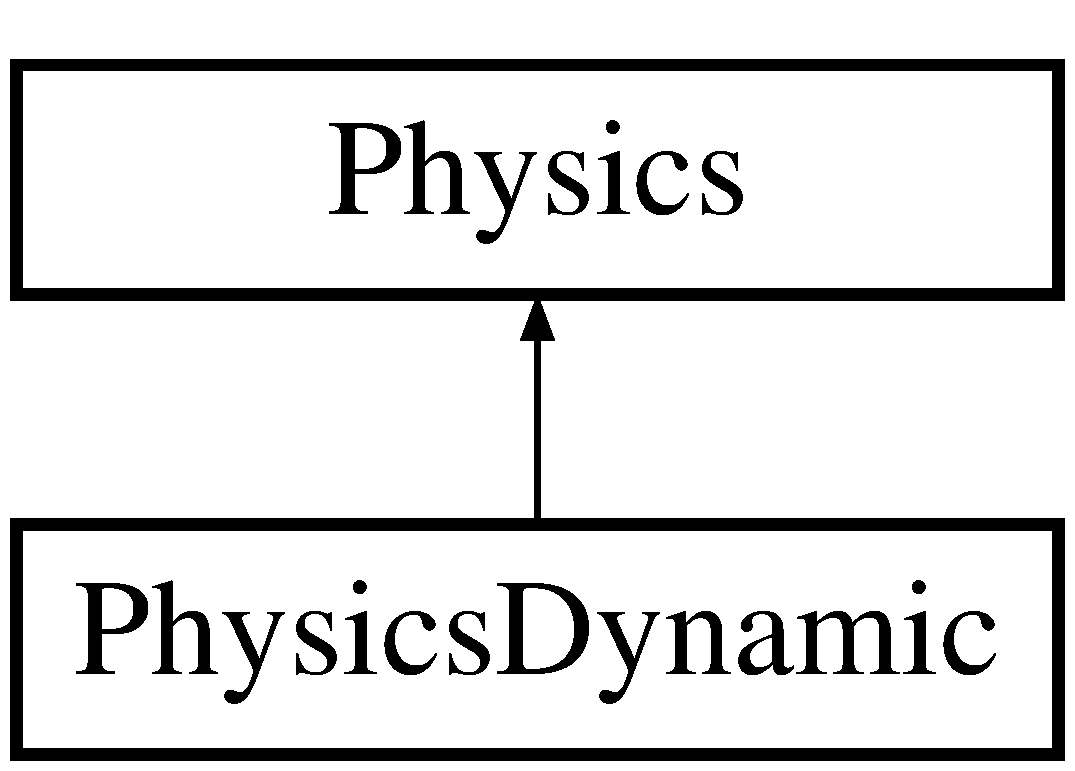
\includegraphics[height=2.000000cm]{class_physics_dynamic}
\end{center}
\end{figure}
\subsection*{Public Member Functions}
\begin{DoxyCompactItemize}
\item 
\hyperlink{class_physics_dynamic_ae6d76e93d11871334b4481f47603705b}{Physics\+Dynamic} (b2\+World world, float x, float y, float width, float height)
\begin{DoxyCompactList}\small\item\em Creates a Dynamic body using the base \hyperlink{class_physics}{Physics} class. \end{DoxyCompactList}\end{DoxyCompactItemize}
\subsection*{Additional Inherited Members}


\subsection{Constructor \& Destructor Documentation}
\mbox{\Hypertarget{class_physics_dynamic_ae6d76e93d11871334b4481f47603705b}\label{class_physics_dynamic_ae6d76e93d11871334b4481f47603705b}} 
\index{Physics\+Dynamic@{Physics\+Dynamic}!Physics\+Dynamic@{Physics\+Dynamic}}
\index{Physics\+Dynamic@{Physics\+Dynamic}!Physics\+Dynamic@{Physics\+Dynamic}}
\subsubsection{\texorpdfstring{Physics\+Dynamic()}{PhysicsDynamic()}}
{\footnotesize\ttfamily Physics\+Dynamic\+::\+Physics\+Dynamic (\begin{DoxyParamCaption}\item[{b2\+World}]{world,  }\item[{float}]{x,  }\item[{float}]{y,  }\item[{float}]{width,  }\item[{float}]{height }\end{DoxyParamCaption})}



Creates a Dynamic body using the base \hyperlink{class_physics}{Physics} class. 


\begin{DoxyParams}{Parameters}
{\em b2\+World} & world \\
\hline
{\em float} & x \\
\hline
{\em float} & y \\
\hline
{\em float} & width \\
\hline
{\em float} & height \\
\hline
\end{DoxyParams}


The documentation for this class was generated from the following files\+:\begin{DoxyCompactItemize}
\item 
Physics\+Dynamic.\+h\item 
Physics\+Dynamic.\+cpp\end{DoxyCompactItemize}

\hypertarget{class_resource_manager}{}\section{Resource\+Manager Class Reference}
\label{class_resource_manager}\index{Resource\+Manager@{Resource\+Manager}}
\subsection*{Public Member Functions}
\begin{DoxyCompactItemize}
\item 
\mbox{\Hypertarget{class_resource_manager_a3b32babd2e81909bbd90d7f2d566fadb}\label{class_resource_manager_a3b32babd2e81909bbd90d7f2d566fadb}} 
\hyperlink{class_resource_manager_a3b32babd2e81909bbd90d7f2d566fadb}{Resource\+Manager} ()
\begin{DoxyCompactList}\small\item\em Constructor of resource manager. \end{DoxyCompactList}\item 
\mbox{\Hypertarget{class_resource_manager_a671c186e4630599e7e36d000c53eaf80}\label{class_resource_manager_a671c186e4630599e7e36d000c53eaf80}} 
\hyperlink{class_resource_manager_a671c186e4630599e7e36d000c53eaf80}{$\sim$\+Resource\+Manager} ()
\begin{DoxyCompactList}\small\item\em deconstructor of resource manager \end{DoxyCompactList}\item 
const sf\+::\+Texture \& \hyperlink{class_resource_manager_abdcc5ba3056bf5ecd282fd6a3249da67}{get\+Texture} (const std\+::string \&filename)
\begin{DoxyCompactList}\small\item\em Pull a texture file. \end{DoxyCompactList}\item 
const sf\+::\+Sound\+Buffer \& \hyperlink{class_resource_manager_a7804aec5b1d1c5c196db33c23eab4153}{get\+Audio} (const std\+::string \&filename)
\begin{DoxyCompactList}\small\item\em Pull an audio file. \end{DoxyCompactList}\item 
sf\+::\+Music \& \hyperlink{class_resource_manager_aae797e6ff05c541b9d880669d4817fb7}{get\+Music} (const std\+::string \&filename)
\begin{DoxyCompactList}\small\item\em Pull a music file. \end{DoxyCompactList}\item 
void \hyperlink{class_resource_manager_a8203e72ff90185317afb3de075c3a687}{delete\+Sound} (const std\+::string \&filename)
\begin{DoxyCompactList}\small\item\em Delete a loaded sound based on the name of the file. \end{DoxyCompactList}\item 
void \hyperlink{class_resource_manager_a77f65cbaa94708fd7a5a17e5991dc22d}{delete\+Sound} (const sf\+::\+Sound\+Buffer \&sound)
\begin{DoxyCompactList}\small\item\em Delete a loaded sound based on the address of the file. \end{DoxyCompactList}\item 
void \hyperlink{class_resource_manager_a7c2f6f0c696844f4e425a38d34b06cee}{delete\+Texture} (const sf\+::\+Texture \&texture)
\begin{DoxyCompactList}\small\item\em Delete a texture based on the address of the texture file. \end{DoxyCompactList}\item 
void \hyperlink{class_resource_manager_a35dd2d508c5170c929b045b8f5b75c10}{delete\+Texture} (const std\+::string \&filename)
\begin{DoxyCompactList}\small\item\em Delete a texture based on the file name. \end{DoxyCompactList}\item 
void \hyperlink{class_resource_manager_aed7bd28f1f13ec392eac7d8d5dd39d6f}{add\+Resource\+Directory} (const std\+::string \&directory)
\begin{DoxyCompactList}\small\item\em Add a new directory for the external files. \end{DoxyCompactList}\item 
void \hyperlink{class_resource_manager_a38fde2e7c5145472f504a6abb06d7a23}{remove\+Resource\+Directory} (const std\+::string \&directory)
\begin{DoxyCompactList}\small\item\em Delete a user generated directory. \end{DoxyCompactList}\end{DoxyCompactItemize}


\subsection{Member Function Documentation}
\mbox{\Hypertarget{class_resource_manager_aed7bd28f1f13ec392eac7d8d5dd39d6f}\label{class_resource_manager_aed7bd28f1f13ec392eac7d8d5dd39d6f}} 
\index{Resource\+Manager@{Resource\+Manager}!add\+Resource\+Directory@{add\+Resource\+Directory}}
\index{add\+Resource\+Directory@{add\+Resource\+Directory}!Resource\+Manager@{Resource\+Manager}}
\subsubsection{\texorpdfstring{add\+Resource\+Directory()}{addResourceDirectory()}}
{\footnotesize\ttfamily void Resource\+Manager\+::add\+Resource\+Directory (\begin{DoxyParamCaption}\item[{const std\+::string \&}]{directory }\end{DoxyParamCaption})}



Add a new directory for the external files. 


\begin{DoxyParams}{Parameters}
{\em const} & std\+::string directory \\
\hline
\end{DoxyParams}
\mbox{\Hypertarget{class_resource_manager_a8203e72ff90185317afb3de075c3a687}\label{class_resource_manager_a8203e72ff90185317afb3de075c3a687}} 
\index{Resource\+Manager@{Resource\+Manager}!delete\+Sound@{delete\+Sound}}
\index{delete\+Sound@{delete\+Sound}!Resource\+Manager@{Resource\+Manager}}
\subsubsection{\texorpdfstring{delete\+Sound()}{deleteSound()}\hspace{0.1cm}{\footnotesize\ttfamily [1/2]}}
{\footnotesize\ttfamily void Resource\+Manager\+::delete\+Sound (\begin{DoxyParamCaption}\item[{const std\+::string \&}]{filename }\end{DoxyParamCaption})}



Delete a loaded sound based on the name of the file. 


\begin{DoxyParams}{Parameters}
{\em const} & std\+::string filename \\
\hline
\end{DoxyParams}
\mbox{\Hypertarget{class_resource_manager_a77f65cbaa94708fd7a5a17e5991dc22d}\label{class_resource_manager_a77f65cbaa94708fd7a5a17e5991dc22d}} 
\index{Resource\+Manager@{Resource\+Manager}!delete\+Sound@{delete\+Sound}}
\index{delete\+Sound@{delete\+Sound}!Resource\+Manager@{Resource\+Manager}}
\subsubsection{\texorpdfstring{delete\+Sound()}{deleteSound()}\hspace{0.1cm}{\footnotesize\ttfamily [2/2]}}
{\footnotesize\ttfamily void Resource\+Manager\+::delete\+Sound (\begin{DoxyParamCaption}\item[{const sf\+::\+Sound\+Buffer \&}]{sound }\end{DoxyParamCaption})}



Delete a loaded sound based on the address of the file. 


\begin{DoxyParams}{Parameters}
{\em const} & sf\+::\+Sound\+Buffer sound \\
\hline
\end{DoxyParams}
\mbox{\Hypertarget{class_resource_manager_a7c2f6f0c696844f4e425a38d34b06cee}\label{class_resource_manager_a7c2f6f0c696844f4e425a38d34b06cee}} 
\index{Resource\+Manager@{Resource\+Manager}!delete\+Texture@{delete\+Texture}}
\index{delete\+Texture@{delete\+Texture}!Resource\+Manager@{Resource\+Manager}}
\subsubsection{\texorpdfstring{delete\+Texture()}{deleteTexture()}\hspace{0.1cm}{\footnotesize\ttfamily [1/2]}}
{\footnotesize\ttfamily void Resource\+Manager\+::delete\+Texture (\begin{DoxyParamCaption}\item[{const sf\+::\+Texture \&}]{texture }\end{DoxyParamCaption})}



Delete a texture based on the address of the texture file. 


\begin{DoxyParams}{Parameters}
{\em const} & sf\+::\+Texture texture \\
\hline
\end{DoxyParams}
\mbox{\Hypertarget{class_resource_manager_a35dd2d508c5170c929b045b8f5b75c10}\label{class_resource_manager_a35dd2d508c5170c929b045b8f5b75c10}} 
\index{Resource\+Manager@{Resource\+Manager}!delete\+Texture@{delete\+Texture}}
\index{delete\+Texture@{delete\+Texture}!Resource\+Manager@{Resource\+Manager}}
\subsubsection{\texorpdfstring{delete\+Texture()}{deleteTexture()}\hspace{0.1cm}{\footnotesize\ttfamily [2/2]}}
{\footnotesize\ttfamily void Resource\+Manager\+::delete\+Texture (\begin{DoxyParamCaption}\item[{const std\+::string \&}]{filename }\end{DoxyParamCaption})}



Delete a texture based on the file name. 


\begin{DoxyParams}{Parameters}
{\em const} & std\+::string filename \\
\hline
\end{DoxyParams}
\mbox{\Hypertarget{class_resource_manager_a7804aec5b1d1c5c196db33c23eab4153}\label{class_resource_manager_a7804aec5b1d1c5c196db33c23eab4153}} 
\index{Resource\+Manager@{Resource\+Manager}!get\+Audio@{get\+Audio}}
\index{get\+Audio@{get\+Audio}!Resource\+Manager@{Resource\+Manager}}
\subsubsection{\texorpdfstring{get\+Audio()}{getAudio()}}
{\footnotesize\ttfamily const sf\+::\+Sound\+Buffer \& Resource\+Manager\+::get\+Audio (\begin{DoxyParamCaption}\item[{const std\+::string \&}]{filename }\end{DoxyParamCaption})}



Pull an audio file. 


\begin{DoxyParams}{Parameters}
{\em const} & std\+::string filename \\
\hline
\end{DoxyParams}
\begin{DoxyReturn}{Returns}
Returns audio file 
\end{DoxyReturn}
\mbox{\Hypertarget{class_resource_manager_aae797e6ff05c541b9d880669d4817fb7}\label{class_resource_manager_aae797e6ff05c541b9d880669d4817fb7}} 
\index{Resource\+Manager@{Resource\+Manager}!get\+Music@{get\+Music}}
\index{get\+Music@{get\+Music}!Resource\+Manager@{Resource\+Manager}}
\subsubsection{\texorpdfstring{get\+Music()}{getMusic()}}
{\footnotesize\ttfamily sf\+::\+Music \& Resource\+Manager\+::get\+Music (\begin{DoxyParamCaption}\item[{const std\+::string \&}]{filename }\end{DoxyParamCaption})}



Pull a music file. 


\begin{DoxyParams}{Parameters}
{\em const} & std\+::string filename \\
\hline
\end{DoxyParams}
\begin{DoxyReturn}{Returns}
Returns music file 
\end{DoxyReturn}
\mbox{\Hypertarget{class_resource_manager_abdcc5ba3056bf5ecd282fd6a3249da67}\label{class_resource_manager_abdcc5ba3056bf5ecd282fd6a3249da67}} 
\index{Resource\+Manager@{Resource\+Manager}!get\+Texture@{get\+Texture}}
\index{get\+Texture@{get\+Texture}!Resource\+Manager@{Resource\+Manager}}
\subsubsection{\texorpdfstring{get\+Texture()}{getTexture()}}
{\footnotesize\ttfamily const sf\+::\+Texture \& Resource\+Manager\+::get\+Texture (\begin{DoxyParamCaption}\item[{const std\+::string \&}]{filename }\end{DoxyParamCaption})}



Pull a texture file. 


\begin{DoxyParams}{Parameters}
{\em const} & std\+::string filename \\
\hline
\end{DoxyParams}
\begin{DoxyReturn}{Returns}
Returns texture 
\end{DoxyReturn}
\mbox{\Hypertarget{class_resource_manager_a38fde2e7c5145472f504a6abb06d7a23}\label{class_resource_manager_a38fde2e7c5145472f504a6abb06d7a23}} 
\index{Resource\+Manager@{Resource\+Manager}!remove\+Resource\+Directory@{remove\+Resource\+Directory}}
\index{remove\+Resource\+Directory@{remove\+Resource\+Directory}!Resource\+Manager@{Resource\+Manager}}
\subsubsection{\texorpdfstring{remove\+Resource\+Directory()}{removeResourceDirectory()}}
{\footnotesize\ttfamily void Resource\+Manager\+::remove\+Resource\+Directory (\begin{DoxyParamCaption}\item[{const std\+::string \&}]{directory }\end{DoxyParamCaption})}



Delete a user generated directory. 


\begin{DoxyParams}{Parameters}
{\em const} & std\+::string directory \\
\hline
\end{DoxyParams}


The documentation for this class was generated from the following files\+:\begin{DoxyCompactItemize}
\item 
Resource\+Manager.\+h\item 
Resource\+Manager.\+cpp\end{DoxyCompactItemize}

%--- End generated contents ---

% Index
\backmatter
\newpage
\phantomsection
\clearemptydoublepage
\addcontentsline{toc}{chapter}{Index}
\printindex

\end{document}
